\documentclass[12pt,a4paper,oneside]{article}
\usepackage[utf8]{inputenc}
\usepackage[acronym, toc, nonumberlist, nogroupskip]{glossaries}

\usepackage[english, polish]{babel}
\usepackage[OT4]{fontenc}
\usepackage{lmodern}
\usepackage{textcomp, gensymb}

%%% fix for \lll
\let\babellll\lll
\let\lll\relax

\usepackage{amsmath}
\usepackage{mathtools}
\usepackage{amsfonts}
\usepackage{fancyhdr}
\usepackage{graphicx}
\usepackage{subfig}
\graphicspath{ {images/} }
\usepackage{amssymb}

%%% fix for \lll
\let\mathlll\lll
\let\lll\babellll

\usepackage[nottoc]{tocbibind}
\usepackage{bm}
\makenoidxglossaries
\usepackage{filecontents}
\glsnoexpandfields
\usepackage[numbers]{natbib}

\setlength\headheight{15pt}
\enlargethispage*{0.7\baselineskip}


\pagestyle{fancy}
\fancyhf{}
\rhead{MICHALSKI Sz.}
\lhead{Star-tracker for Cubesat satellites}
%\lhead{Star-tracker dla Cubesat'ów}
\rfoot{\thepage}

\author{Szymon MICHALSKI}
\title{PROGRAM STAR-TRACKER DLA SATELITÓW TYPU CUBE-SAT}


\begin{filecontents}{gloss.tex}
%================ACRONYMS=================%
\newacronym{leo}{LEO}{Low Earth Orbit}
\newacronym{adcs}{ADCS}{Attitude Determination and Control System}
\newacronym{lis}{LIS}{Lost-In-Space}
\newacronym{gps}{GPS}{Global Positioning System}
%================SYMBOLS=================%
\newglossaryentry{phi}{type=symbols, name=$\phi$, sort=phi, description={Euler angle, roll}}
\newglossaryentry{theta}{type=symbols, name=$\theta$, sort=theta, description={Euler angle, pitch}}
\newglossaryentry{psi}{type=symbols, name=$\psi$, sort=psi, description={Euler angle, yaw}}
\newglossaryentry{euler_rotation_matrix}{type=symbols, name=$\bm{R}(\cdot)$, sort=euler_rotation_matrix, description={Rotation matrix using Euler angles}}
\newglossaryentry{unit_quaterion}{type=symbols, name=$\bm{q}$, sort=unit_quaterion, description={Unit quaternion}}
\newglossaryentry{scalar_quaternion_part}{type=symbols, name=$q_0$, sort=sigma, description={Scalar part of unit quaternion}}
\newglossaryentry{vector_quaternion_part}{type=symbols, name=$\bm{q}_{vec}$, sort=scalar_quaternion_part, description={Vector part of unit quaternion}}
\newglossaryentry{quaternion_matrix}{type=symbols, name=$\bm{Q}$, sort=quaternion_matrix, description={Quaternion matrix}}
\newglossaryentry{general_euler_angle}{type=symbols, name=$v$, sort=general_euler_angle, description={General Euler angle}}
\newglossaryentry{unit_vector}{type=symbols, name=$\bm{n}$, sort=unit_vector, description={Unit vector}}
\newglossaryentry{identity_matrix}{type=symbols, name=$\bm{I}$, sort=identity_matrix, description={Identity matrix}}
\newglossaryentry{skew_symmetrix_matrix}{type=symbols, name=$\bm{S}(\cdot)$, sort=skew_symmetrix_matrix, description={Skew symmetric matrix}}
\newglossaryentry{rotation_matrix}{type=symbols, name=$\bm{R}_n^b$, sort=rotation_matrix, description={Rotation matrix representing a rotation from n to b}}
\newglossaryentry{least_squares_estimate_rotation_matrix}{type=symbols, name=$\bm{M}$, sort=least_squares_estimate_rotation_matrix, description={Least squares estimate of rotation matrix}}
\newglossaryentry{unit_vector_ned}{type=symbols, name=$\bm{r}$, sort=unit_vector_ned, description={Known directional unit vector in the NED frame}}
\newglossaryentry{unit_vector_body}{type=symbols, name=$\bm{b}$, sort=unit_vector_body, description={Known directional unit vector in the BODY frame}}

\end{filecontents}

\newglossary{symbols}{sym}{sbl}{List of Symbols}
\makenoidxglossaries
\glsnoexpandfields
\loadglsentries{gloss.tex}


\begin{document}
\selectlanguage{english}

\begin{titlepage}
	\centering

	INSTITUTE OF CONTROL AND COMPUTATION ENGINEERING\par
	FACULTY OF ELECTRONICS AND INFORMATION TECHNOLOGY\par
	WARSAW UNIVERSITY OF TECHNOLOGY\par
%	INSTYTUT AUTOMATYKI I INFORMATYKI STOSOWANEJ\par
%	WYDZIAŁ ELEKTRONIKI I TECHNIK INFORMATYJNYCH\par
%	POLITECHNIKA WARSZAWSKA\par
	\vspace{0.5cm}
	
\includegraphics[scale=0.3]{logo_WEiTI.jpg}
	\hspace{1cm}
	
\includegraphics[scale=0.2]{Logo-PW-duze.jpg}
	\hspace{1cm}
	
\includegraphics[scale=1]{ia_600_600.png}
	\par
	\vspace{2cm}
	MASTER OF SCIENCE THESIS\par
%	MAGISTERSKA PRACA DYPLOMOWA\par
	\vspace{0.2cm}
	{\huge STAR-TRACKER PROGRAM FOR CUBESAT SATELLITES\par}
%	{\huge PROGRAM STAR-TRACKER DLA SATELITÓW TYPU CUBE-SAT\par}
	\vspace{0.2cm}
	{\large Szymon MICHALSKI\par}
	\vspace{3cm}
	\begin{flushright}
	Supervisor:\par
%	Promotor:\par
	prof. dr hab. inż. Ryszard Romaniuk\par
	\end{flushright}
	\vspace{6cm}
	{\large Warszawa 2017\par}
\end{titlepage}

\pagenumbering{arabic}
\setcounter{page}{2}
\newpage
\begin{abstract}
Last years directed space industry towards small satellites. Many countries which did not have possibility to enter this branch of industry before now create their own solutions. The goal of this work is to create fully functioning star-tracker software eligible to be used in future satellites as Polish solution of determination of satellite attitude towards Earth. Work contains also description of individual parts and variants of solutions connected with star-tracker.
\end{abstract}
\newpage
\begin{otherlanguage}{polish}
\begin{abstract}
Ostatnie lata ukierunkowały przemysł kosmiczny na małe satelity. Wiele krajów, które wcześniej nie miały możliwości wejścia w tę gałąź przemysłu, teraz tworzą własne rozwiązania. Celem niniejszej pracy dyplomowej jest stworzenie w pełni działającego oprogramowania star-trackera nadającego się do wykorzystania w przyszłych satelitach jako polskie rozwiązanie problemu określania orientacji satelity względem ziemi. Praca zawiera też opis poszczególnych części i wariantów rozwiazania problemów związanych ze star-trackerem.
\end{abstract}
\end{otherlanguage}
\newpage

\tableofcontents

\newpage
\setlength{\parindent}{1cm}
\setlength{\parskip}{\baselineskip}%



\glsaddall
\setlength{\glsdescwidth}{0.5\linewidth}
\setlength{\glspagelistwidth}{0.1\linewidth}

\printnoidxglossary[type=acronym,sort=letter]
\newpage

\printnoidxglossary[type=symbols,sort=use]

\newpage
\citet{jenssen2011comparison}
\citet{valenti2015keeping}
\citet{delabie2012highly}
\citet{jalabert2011optimization}
\citet{felikson2011orbit}
\citet{knutson2012fast}
\citet{rose2003star}
\citet{mortari2002starnav}


\section{Introduction}
Stars were used for navigation already ages ago. Together with technological development, spread of sailing and seafaring people started to use more advanced tools helping to more precisely estimate position of ships on sea. In XVIII century new tool was created, named sextant. This device helped to quite precisely calculate angle between the line ship-horizon and ship-star, what let to estimate position.

Nowadays, hundreds of years later, thanks to other technologies like for example Global Positioning System (GPS) stars are not necessary any more for travelling. As it is commonly known, GPS technology is based on satellites, and today those satellites need stars for determining their attitude towards Earth.

With the miniaturization of electronics and batteries new type of satellites was invented: CubeSat micro-satellite. They have now greater sensory and processing power possibilities, previously found only in larger satellites. However CubSats are still behind in terms of attitude determination.

\subsection{Motivation}
The goal of this work is to make fully operational star-tracker software, that could be used on Cubesat satellites. Such program could be used on space missions and could start Polish state-of-the-art technology in growing space technology sector.
There is already existing prototype of on-board computer for such CubeSat satellite, which together with this work should create full star-tracker device: hardware + software.

\subsection{Outline of thesis}

This thesis consists of several chapters. Here they are shortly summarized:\par
\setlength{\parindent}{0cm}
\textbf{Chapter 1} serves as introduction to this thesis and describes the motivation and goal of this work. It also describes the background of the topic.\par
\textbf{Chapter 2} describes all the important foundations for the fully understanding given work.\par
\textbf{Chapter 3} is the main part of this thesis. It describes how the star-tracker program works and goes through detailed comparison of different approaches.\par
\textbf{Chapter 4} describes the created prototype of star-tracker in Python language.\par
\textbf{Chapter 5} talks about the implementation of star-tracker on the existing prototype of on-board computer.\par
\textbf{Chapter 6} describes how the finished program is performing.\par
\textbf{Chapter 7} contains conclusions about this work and created star-tracker program.\par

\setlength{\parindent}{1cm}

\subsection{Similar work}

There exists a number of works connected to topic of star-tracker. Many works are cited later in this thesis as they describe important parts of algorithms. There are just a few works dealing with whole start-tracker program, not just parts of it, and nearly no works about whole program together with implementation on the real equipment.

\subsection{Cubesat}


In recent years there has been the development of micro-satellites called CubeSats. CubeSat is a standard created in 1999 at the California Polytechnic State University \cite{heidt2000cubesat}, which is used for low-cost micro-satellites. CubeSats are measured in units. Most are 1U, 2U and 3U. CubeSat 1U has a size of 10 cm on each edge and the maximum weight of 1.333 kg, while the CubeSat 2U is 20x10x10 cm and can weigh up to 2.666 kg.

The advantage of the standard is primarily reduction of the price of elevation of such satellites into orbit. Their popularity is evidenced by the fact that the percentage of satellites weighing less than 10 kg has increased to about 60\% of all satellites, and only CubeSats make up about half of the small satellites that were launched in last years \cite{swartwout2011brief}. Till now there were around 800 CubeSats launched \cite{nanosats}.

There exist wide range of CubeSat examples. Mostly they are scientific and students' satellites, for learning, experimental and science purposes. There are also few Polish examples: PW-SAT (1U) and PW-SAT 2 (2U) designed by students of Warsaw University of Technology, and Lem (8U) and Heweliusz (8U), both made at Polish Academy of Sciences. PW-SAT and PW-SAT 2 were used for learning and experimenting with new technologies, like deorbitation sail, solar sensor, etc. \cite{pw-sat2}.
Scientific satellites Lem and Heweliusz were built as part of BRITE programme - joint programme of Austria, Canada and Poland. The goal of this programme is to research mechanisms of energy transportation and angular momentum which happen inside hottest stars \cite{brite-pl}.

Typical CubeSat consist of many different components. Quite often it has antennas and radios for communication with mission centre on Earth, Electric Power System (EPS - subsystem responsible for managing electric power in the satellite), Attitude Determination and Control (ADCS - subsystem responsible for analysing data from sensors and taking decision about trajectory, etc.), magnetometer, star-tracker, sun sensors, payload processor with mission instructions, etc. CubeSats are quite small, hence they usually do not have any propulsion system. Figure \ref{fig:cubesat-build} shows the components of CubeSat on example of NASA's Interplanetary NanoSpacecraft Pathfinder In a Relevant Environment (INSPIRE).

\begin{figure}[!htbp]
  \centering
  \subfloat[PW-SAT \cite{pw-sat-image}]{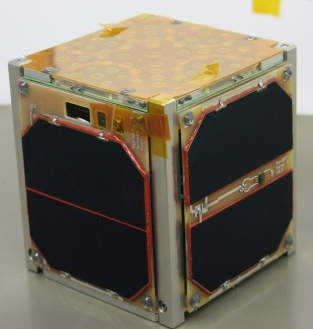
\includegraphics[width=0.4\textwidth]{pw-sat.jpg}\label{fig:pw-sat}}
  \hfill
  \subfloat[PW-SAT 2 \cite{pw-sat2}]{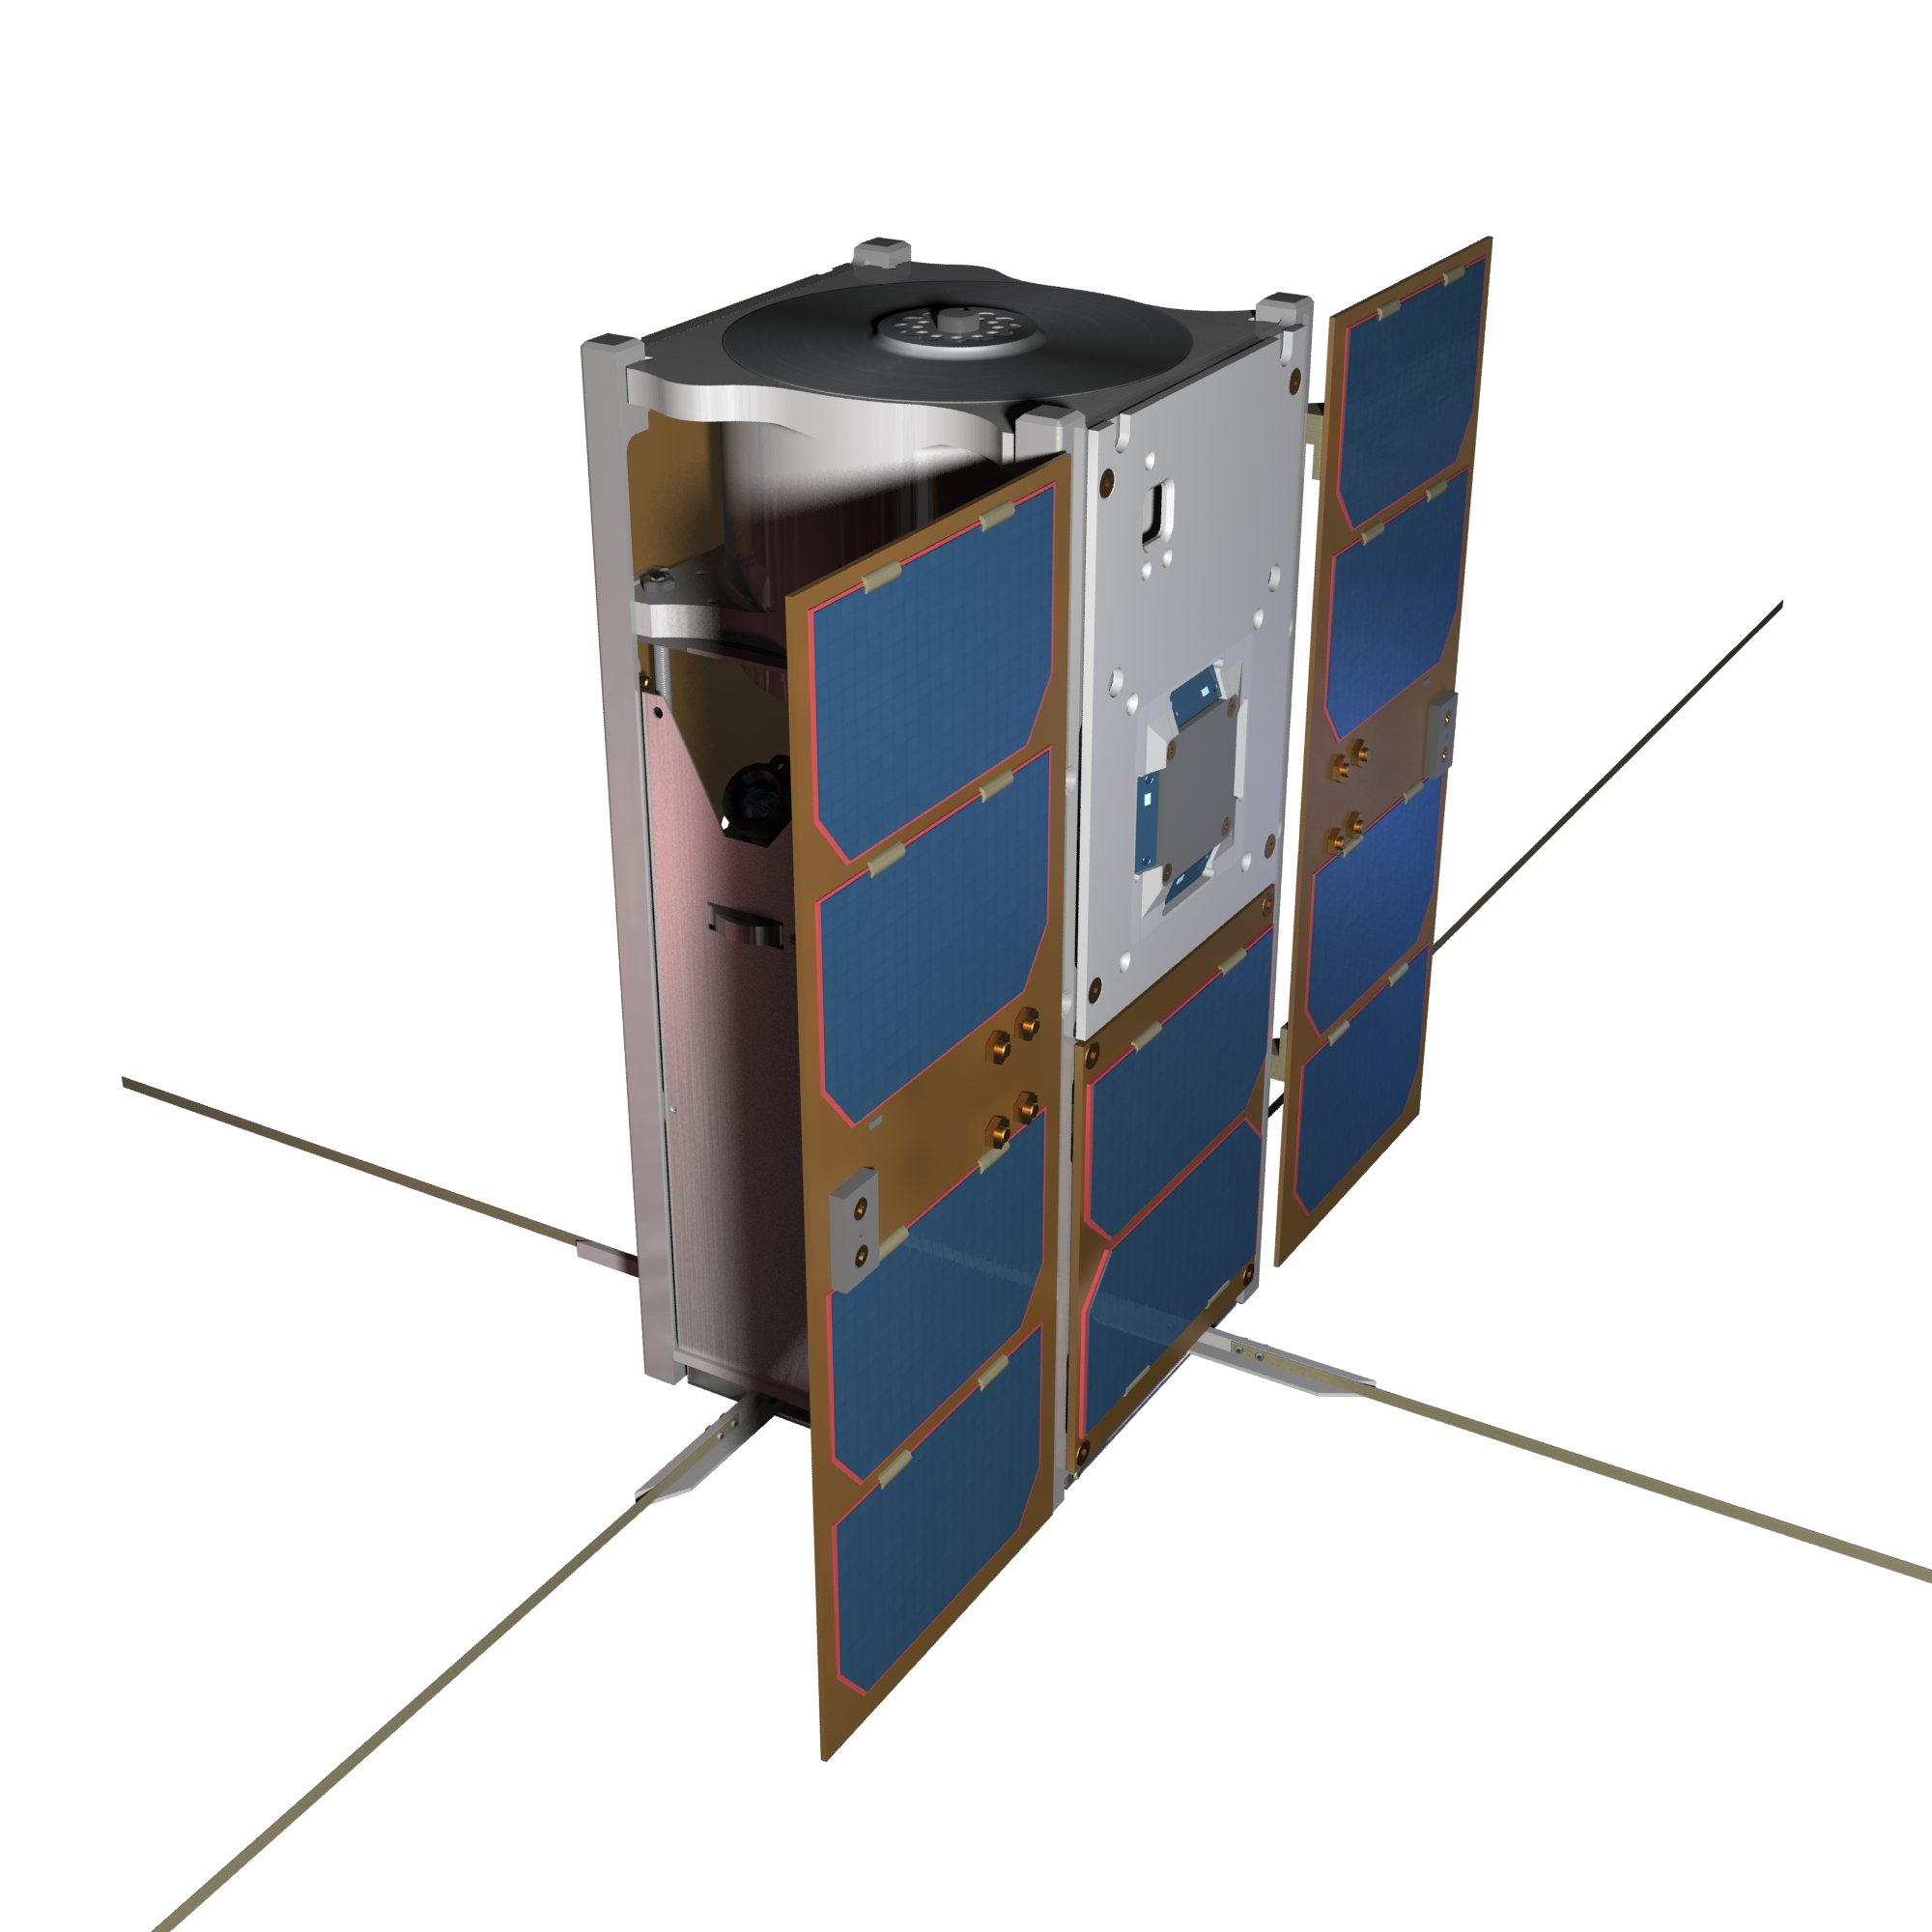
\includegraphics[width=0.5\textwidth]{PW-Sat2_2016_16_MSwietlik.png}\label{fig:pw-sat2}}
  \hfill
  \subfloat[BRITE-PL (Lem, Heweliusz) \cite{brite-pl-gunter}]{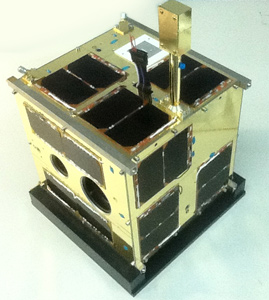
\includegraphics[width=0.5\textwidth]{brite.jpg}\label{fig:brite}}
  \caption{Example of Polish CubeSats.}
  \label{fig:satellites-examples}
\end{figure}


\begin{figure}[ht]
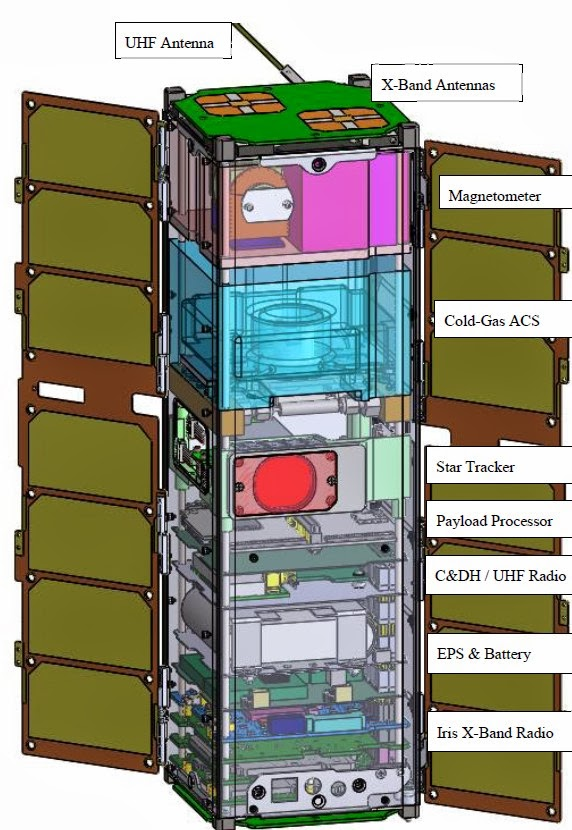
\includegraphics[scale=0.45]{INSPIRE_JPL.jpg}
\centering
\caption{CubeSat build - INSPIRE, Image \cite{cubesat-build}}
\label{fig:cubesat-build}
\end{figure}

Costs of such CubeSat satellite on example of PW-SAT 2: 120,000-200,000 EUR for putting the satellite on the orbit and round 70,000 EUR for designing and building the satellite itself \cite{pw-pw-sat2}.


\subsection{Means of attitude determination}

Attitude of spaceships must be usually stabilised and controlled for various reasons.
It is necessary for satellite antenna to be pointing towards Earth for the proper communication, to intelligently control the heat by using the effects of cooling and heating of the shadows and sunlight, as well as to navigate: manoeuvres must be performed in the right direction.

Attitude is determined between two coordinate systems (where one is reference system) and defines by what angles the coordinate system connected with the researched object has to be shifted in order to cover the reference system.
Devices such as planes and satellites have so called Attitude Determination and Control System (ADCS), which controls attitude of object relative to an inertial reference frame or another entity (the celestial sphere, certain areas, the nearby objects, etc.).

Currently, attitude determination of CubeSats is limited mainly to the sun sensors, magnetometers and measurements of inertia. The following table describes the accuracy of different sensors. Unquestionably winner here is the star-tracker, which, due to its quality and uniqueness of the constellations is ideal for navigation. 

\subsubsection{Inertial Measurement Unit}
\subsubsection{Sun Sensors}
\subsubsection{Star Sensors}
\subsubsection{Horizon Sensors}
\subsubsection{Magnetometer}
\subsubsection{GPS - maybe}
\subsubsection{Conclusions}
Sun sensors can provide very accurate measurements, but can only operate in sunlight. For low-Earth orbit (LEO), even 30\% of the orbit can be done in the darkness. Magnetometers are small and can give accurate measurements of the proper calibration. Their drawback is the limited knowledge of the magnetic field and electromagnetic interference due to highly integrated construction of CubeSats.
Microelectromechanical gyroscopes are small enough to fit into a CubeSats. However, they suffer from sudden movements, and could not maintain the correct measurement of the 15-minute period of the eclipse orbit LEO. To be truly competitive and reliable platform, CubeSats must provide the correct determination of attitude. The best way to meet this goal is by using star-trackers.

\citet{larson1992space}
\citet{lima2000comparison}

\renewcommand{\arraystretch}{1.5}
\begin{table}[ht]
\begin{tabular}{|p{4.5cm}|p{8cm}|}
\hline 
Sensor & Typical Performance Range \\ 
\hline 
Inertial \newline Measurement Unit \newline (Gyros and Accelerometers) & Gyro drift rate = 0.003 deg/hr to 1 deg/hr,\newline accel. \newline Linearity = 1 to 5 x $10^{-6} g/g^2$ over range\newline of 20 to 60 g \\ 
\hline 
Sun Sensors & Accuracy = 0.005 deg to 3 deg \\ 
\hline 
Star Sensors\newline (Scanners and Mappers) & Attitude accuracy = 1 arc sec to 1 arc min \newline 0.0003 deg to 0.01 deg \\ 
\hline 
Horizon Sensors\newline -Scanner/Pipper\newline -Fixed Head (Static) & Attitude accuracy: \newline 0.1 deg to 1 deg (LEO) \newline $<0.1$ deg to 0.25 deg \\ 
\hline 
Magnetometer & Attitude accuracy = 0.5 deg to 3 deg \\ 
\hline 
\end{tabular}
\caption{Sensor Accuracy Ranges. Adapted from \citet{larson1992space}}
\end{table}

\begin{table}[h!bt]
\begin{tabular}{|p{3cm}|p{3.3cm}|p{6cm}|}
\hline
\textbf{Sensor} & \textbf{Accuracy} & \textbf{Characteristics \newline and Applicability} \\ 
\hline
Magnetometers & 1.0\degree (5000km alt) \newline 5.0\degree (200 km alt) & Attitude measured relative to \newline Earth’s local magnetic field. \newline Magnetic field uncertainties and \newline variability dominate accuracy. \newline Usable only below $\approx$6,000 km. \\ 
Earth sensors & 0.05\degree (GEO) \newline 0.1\degree (LEO) & Horizon uncertainties dominate \newline accuracy. Highly accurate units \newline use scanning. \\ 
Sun sensors & 0.01\degree & Typical field of view +-30\degree \\ 
Star sensors & 2 arc-sec & Typical field of view +-6\degree \\ 
Gyroscopes & 0.001 deg/hr & Normal use involves periodically resetting reference. \\ 
Directional \newline antennas & 0.01\degree to 0.5\degree & Typically 1 of the antenna \newline beam width \\
\hline
\end{tabular} 
\caption{Sensor Accuracy Ranges. Adapted from \citet{hall2003spacecraft}}
\end{table}

\subsection{On-board computer}
This section will describe the on-board computer which was done as part of other thesis.

\newpage
\section{Preliminaries}
\subsection{Coordinate frames}
\subsubsection{ECI frame}
The Earth Centered Inertial frame has its x-axis pointing towards the vernal equinox, and its z-axis pointing along the rotation axis of the Earth at some initial time. The y-axis completes a right handed orthogonal coordinate system. The frame’s origin is at the center
of the Earth.
\citet{larson1992space}
\begin{figure}[ht]
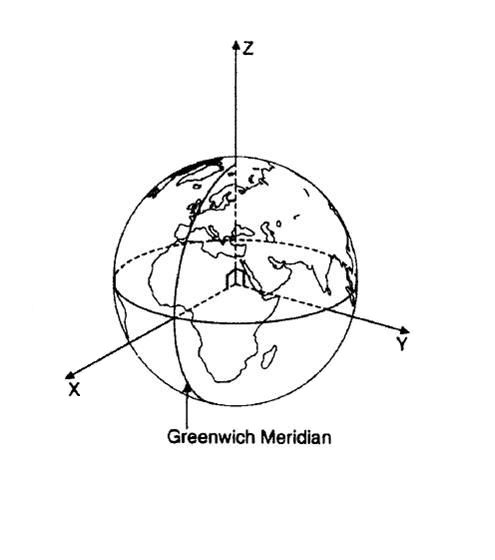
\includegraphics[scale=0.4]{eci_frame.jpg}
\centering
\caption{ECI frame, Image \citet{larson1992space}}
\label{fig:eci_frame}
\end{figure}
\subsubsection{ECEF frame}
This frame also has its origin at the center of the Earth, but the Earth Centered Earth Fixed frame has its x-axis pointing towards the point where the intersection between the longitude and latitude have zero value. It can also be described as the intersection between the Greenwich meridian and the Equator. The frame’s z-axis is pointing along the Earth’s rotation axis. The y-axis completes the right handed orthogonal system. The ECEF frame is not an inertial frame, it rotates relative to the ECI frame along the Earth rotation.
\subsubsection{NED frame}
The North East Down frame has its z-axis pointing downwards, perpendicular to the tangent plane of the Earth’s reference ellipsoid. The ellipsoid is mathematically defined and fitted for approximation of the Earth. The x-axis points towards true north and the y-axis points East. The NED frame is an inertial frame.
\subsubsection{BODY frame}
This frame is attached to the satellite, and is moving and rotating with it. The origin coincides with the origin of the NED frame. The axes coincide with the principle axes of inertia; the x-axis is pointing forwards, the y-axis is pointing to the right side and the
z-axis is pointing downwards through the camera side of the satellite.
\begin{figure}[h]
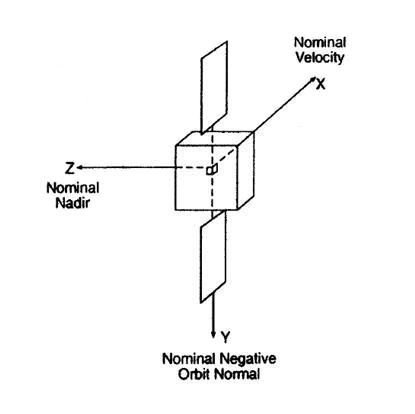
\includegraphics[scale=0.5]{body_frame.jpg}
\centering
\caption{BODY frame, Image \citet{larson1992space}}
\label{fig:body_frame}
\end{figure}
\subsection{Space environment}
\subsection{Attitude representations}
Several representations for describing attitude are available, the most common being Euler angles. More complicated attitude representations are quaternions. Quaternions are used for all the estimation methods presented in this thesis. They are singular-free, and are therefore well suited for attitude determination.
\subsubsection{Euler angles}

%Robot Learning Darmstadt
%Problems with Euler Angles:
%Not Unique: Many angles result in the same rotation
%Hard to quantify differences between two Euler Angles
%Unit-Quaternion
%Solves the problems of singularities with the Euler Angles
%Easier to compute differences of orientations
%Important if we want to control the orientation of the end-effector
%See Siciliano or Spong Textbook!
%https://en.wikipedia.org/wiki/Apparent_magnitude
%Polar moment

Euler angles were first described by Leonhard Euler in 1776, and are used to represent the orientation of a body \citet{euler1775formulae}. Three parameters are required for a full understanding of the
orientation between two frames, one angle for the rotation around each of the axes. The angles are called roll, pitch and yaw and are usually written as phi, ro and psi. The Euler angles are often used for the definition of rotation matrices about the x, y and z-axis. In R 3 , the coordinate system rotations in a counter-clockwise direction looking towards the origin are given from:

\begin{equation}
\bm{R}_x(\phi) = \begin{bmatrix}
1 & 0 & 0 \\
0 & \cos(\phi) & -sin(\phi) \\
0 & \sin(\phi) & \cos(\phi)
\end{bmatrix}
\end{equation}
\begin{equation}
\bm{R}_y(\theta) = \begin{bmatrix}
\cos(\theta) & 0 & \sin(\theta) \\
0 & 1 & 0 \\
-\sin(\theta) & 0 & \cos(\theta)
\end{bmatrix}
\end{equation}
\begin{equation}
\bm{R}_z(\psi) = \begin{bmatrix}
\cos(\psi) & -\sin(\psi) & 0 \\
\sin(\psi) & \cos(\psi) & 0 \\
0 & 0 & 1
\end{bmatrix}
\end{equation}
\subsubsection{Quaternions}
\citet{hamilton1844lxxviii}
\citet{cayley1845xiii}
\citet{courant1953methods}
\citet{mebius2005matrix}
\citet{mathworldconjugate}
\citet{shoemake1985animating}
\citet{horn1987closed}

Quaternions were first described by Sir William Rowan Hamilton in 1843 \citet{hamilton1844lxxviii}. His intension was to find an extension of vector algebra, and in 1845 Arthur Cayley published an article where he used multiplication of quaternions to describe rotations \citet{cayley1845xiii}. Three of the four elements of a quaternion give the coordinates for the axis of rotation, while the fourth is described by the angle of rotation \citet{courant1953methods}.
A quaternion can be written as a four-dimensional vector:
\begin{equation}
\bm{q} \coloneqq \begin{bmatrix}
q_0 \\
q_1 \\
q_2 \\
q_3
\end{bmatrix}
\end{equation}
The real part of the quaternion behaves like a scalar in the three-dimensional vector space.
Using a rotation angle vi, the real part can be written as:
\begin{equation}
q_0 = \cos(v/2)
\end{equation}

\begin{equation}
\bm{n} = \frac{\bm{n}}{||\bm{n}||}
\end{equation}
The imaginary part uses a unit vector given from n = n/||n|| (wzor)
where the norm of the vector, ||n||, is defined as the square root of each of the squared elements of n added together.
Throughout the thesis, vectors and matrices will be written in bold print.
The imaginary part can be written as a vector:
\begin{equation}
\bm{q}_{vec} \coloneqq \begin{bmatrix}
q_1 \\
q_2 \\
q_3
\end{bmatrix}
= [\bm{n}\sin(v/2)]
\end{equation}
There are several ways to write quaternions. Sometimes it is convenient to think of a quaternion as the sum of a scalar and a vector written as:
\begin{equation}
\bm{q} \coloneqq q_0 + \bm{q}_vec = q_0 + q_1i + q_2j+ q_3k
\end{equation}
Complex numbers can be represented as matrices, and so can quaternions. A quaternion describes a point in 4D space, and can be represented by a 4 × 4 matrix by using a left-isoclinic rotation as proved in \citet{mebius2005matrix}, and used in \citet{mathworldconjugate} and \citet{shoemake1985animating}:
\begin{equation}
\bm{Q} = \begin{bmatrix}
q_0 & -q_1 & -q_2 & -q_3 \\
q_1 & q_0 & -q_3 & q_2 \\
q_2 & q_3 & q_0 & -q_1 \\
q_3 & -q_2 & q_1 & q_0
\end{bmatrix}
\end{equation}
The transpose of the matrix is the same as the conjugate of the quaternion:
\begin{equation}
\bm{q}^* \coloneqq q_0 - \bm{q}_{vec} = q_0 + q_1i + q_2j+ q_3k
\end{equation}
Two quaternions are conjugate if they are orthogonal with respect to their inner product \citet{horn1987closed}. The inverse of a quaternion q is defined as q -1 = 1/q . In this report, the mathematics
are based on unit quaternions, which satisfies the constraint:
\begin{equation}
\bm{q}^T\bm{q} = 1
\end{equation}
The length of a unit quaternion is 1, which leads its inverse to be its conjugate.
\subsubsection{Advantages of quaternions}
The unit quaternion notation is compact, and round off errors are easier to handle than for matrix representation. The nearest orthonormal matrix to one that is not quite orthonormal, is difficult to find. Multiplying unit quaternions may similarly lead to quaternions that are no longer of unit length, but these can easily be normalized to make sure they correspond to valid rotations. The computational cost of normalizing a quaternion is much less than
for normalizing a matrix.
Quaternions are safe from a phenomenon called gimbal lock. When the pitch angle in a pitch/roll/yaw-system is rotated 90\degree up or down, and the yaw and roll correspond to the same motion, a degree of freedom of rotation can be lost. In a gimbal-based aerospace inertial navigation system, this could have disastrous results if the aircraft is in a steep dive or ascent \citet{shoemake1985animating}. The quaternion elements vary continuously over the unit sphere in $R^4$ , (denoted by $S^3$ ) as the orientation changes, avoiding this problem.
Due to the possible spin in the CubeSat, combined with the singularity problem for Euler angles, an attitude estimation method based on unit quaternions is preferred.

\newpage
\section{Star-tracker program}

Star-tracker program is designed to determine the attitude of the satellite with the image of the stars made by the satellite camera. Before the start of the mission star catalogue is generated, based on the star catalogues obtained from the observatories on Earth and uploaded to the computer on-board the satellite. 

After the start, the satellite is released from rocket's tank in space and has no idea where it is. Then the star-tracker on the satellite enters into Lost-In-Space mode (LIS) and analyses the current image of the stars of the camera, and then searches the corresponding result of stars in the on-board star catalogue database. If it finds an entry in the database, the satellite goes into tracking mode. This means each next calculation of the orientation of the satellite attitude is going to be based on a comparison of the current pictures of stars with the preceding ones. If it cannot find the result in the database, this action is repeated from time to time, until a match is found in the database and the program will go into tracking mode.

Of course LIS does not happen only at the beginning of the satellite's flight, but can also result from many causes, e.g. a satellite which is for a long time in the darkness may discharge its battery, and during the next entry into sunlit zone will turn on and look again its attitude. Another case is when satellite becomes lost, although once found the orientation and follow her. This happens, because the successive results are based on preceding ones and even the smallest mistake will grow until the satellite will not be able to correctly calculate their attitude. It may also happen that the satellite will rotate around its axis so fast that the program would not keep up with the processing the image and calculations. In this case, the corresponding other satellite's systems should take an action reducing his spin, but this is not part of this work. It is showed in simple conceptual diagram - Figure \ref{fig:startracker_conceptual_alg}.

\begin{figure}[ht]
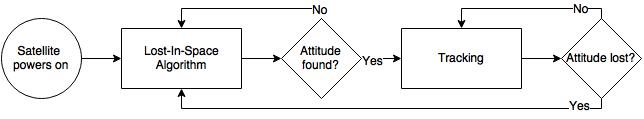
\includegraphics[scale=0.59]{startracker_eng.jpg}
\centering
\caption{Startracker conceptual algorithm diagram}
\label{fig:startracker_conceptual_alg}
\end{figure}

Each part - LIS and tracking - consists of smaller algorithms. Lost-In-Space at the beginning of reading an image from the camera, thresholds the image. Thresholding is basically throwing away parts of the image which do not exceed the threshold brightness, making just bright enough stars taken into account. Next it calculates centroid (center of mass) of selected stars, identifies these stars using one of the possible methods (here Planar Triangle, described later) and searches the directory on-board technology (k-vector).
If the database does not contain corresponding stars, the algorithm returns to the input state and starts analysing the next image. If it manages to find the corresponding stars, the program determines the attitude of the satellite (by what angle is satellite shifted comparing to the referenced object - Earth or previous image) and enters tracking mode. Tracking mode is in large part similar to the LIS. The algorithm also first analyses the photo, selects and calculates centroids stars, identifies them, but does not search for stars in the directory board. In this algorithm are compared two images, one following after the other, and on this basis the current attitude is calculated.
%converts the results of the Cartesian coordinates to the ecliptic (the stars in the directory board are created using images of the Earth, which results in other coordinates) 
%does not transform coordinates, and not available\citet{ju2003overview}\par

Generally star-tracker is divided into three main parts\citet{6187242}:
\begin{itemize}
\item recognising stars on the image and converting the data into list of star vectors by calculating star centroids;
\item identifying which star vector represents which real star in catalogue. This is done by comparing star vectors from the image with data in star catalogue, which is generated before space mission;
\item estimating the attitude by calculating the displacement between two frames.
\end{itemize}

\subsection{Centroid - start recognition}
\citet{samaan2002predictive}

\citet{liebe2002accuracy}


The whole star-tracker program is based on very precise calculations. For this reason, the calculation based on the position of the pixels only can give incorrect results. It is necessary to calculate the position of stars with an accuracy exceeding pixels. This is why the calculation of the star centroids is necessary.

The first step is the determination of stars' position in the plane of the image. If focused star pictures are recorded, the image of each star will fall only on one or two pixels, and most likely the saturate these pixels, resulting in a pixel level accuracy.
Many star-trackers are doing deliberately blurred images, in order to spread the photons on a larger number of pixels, which allows the algorithm for calculating the centroid in sub-pixel accuracy.

After the registration of such image, the centroid of the star is found similarly to the centroid weight points array, with a few differences. Firstly, instead of weight light intensity is used. Secondly, the intensity of light is usually normalized by the pixels around the star in order to filter out glare or noise. The resulting outcome is a series of two-dimensional coordinates on the photo plane with the starting point at the center of the image. This allows the system to the coordinates of the stars can be easily converted into unit vectors in the next step.

The algorithm requires specification of the light intensity threshold (to select the brightest stars) $I_{thresh}$ and the size of the Region of Interest (ROI) $a_{ROI}$ in pixels. These values are adjusted to manipulate the performance of the algorithm. For example, the higher the value of $I_{thresh}$ is more resistant to noise, but can miss some real stars in the picture. Similarly, a large value $a_{ROI}$ means a more exact value of centroid, but the algorithm can see one star there, where are actually two within a short distance of each other. The centroiding part is about trade-off between noise resistance and star recognition, and also between recognizing few close stars as one and recognizing one big star as a few.
Please note that $a_{ROI}$ must be a positive odd number for the proper functioning of the algorithm.


The idea of how to calculate such centroids is adapted from\citet{6187242} and described below:

\begin{equation}
x_{start} = x - \frac{a_{ROI} - 1}{2}
\end{equation}
\begin{equation}
y_{start} = y - \frac{a_{ROI} - 1}{2}
\end{equation}
\begin{equation}
x_{end} = x_{start} + a_{ROI}
\end{equation}
\begin{equation}
y_{end} = y_{start} + a_{ROI}
\end{equation}
\begin{subequations}
\begin{equation}
I_{bottom} = \sum_{i=1}^{x_{end}-1} I(i, y_{start})
\end{equation}
\begin{equation}
I_{top} = \sum_{i=2}^{x_{end}} I(i, y_{end})
\end{equation}
\begin{equation}
I_{left} = \sum_{j=1}^{y_{end}-1} I(x_{start}, j)
\end{equation}
\begin{equation}
I_{right} = \sum_{j=2}^{y_{end}} I(x_{start}, j)
\end{equation}
\begin{equation}
I_{border} = \frac{I_{top} + I_{bottom} + I_{left} + I_{right}}{4(a_{ROI} - 1)}
\end{equation}
\end{subequations}
\begin{equation}
\tilde{I}(x,y) = I(x,y) - I_{border}
\end{equation}

\begin{equation}
B = \sum_{i=x_{start}+1}^{x_{end}-1}\sum_{j=y_{start}+1}^{y_{end}-1}\tilde{I}(i,j)
\end{equation}
\begin{equation}
x_{CM} = \sum_{i=x_{start}+1}^{x_{end}-1}\sum_{j=y_{start}+1}^{y_{end}-1}\frac{i \times \tilde{I}(i,j)}{B}
\end{equation}
\begin{equation}
x_{CM} = \sum_{i=x_{start}+1}^{x_{end}-1}\sum_{j=y_{start}+1}^{y_{end}-1}\frac{j \times \tilde{I}(i,j)}{B}
\end{equation}

\begin{equation}
u = \frac{
\begin{bmatrix}
\mu x_{CM} & \mu y_{CM} & f
\end{bmatrix}
^T}
{||
\begin{bmatrix}
\mu x_{CM} & \mu y_{CM} & f
\end{bmatrix}
||}
\end{equation}

\subsection{Star identification}
all \citet{spratling2009survey}\par
Brightness Independent 4-Star Matching Algorithm for Lost-in-Space 3-Axis Attitude Acquisition\citet{dong2006brightness} \par
SP-Search: A New Algorithm for Star Pattern Recognition \citet{mortari1999sp} \par
Star Identification using Neural networks \citet{miri2012star} \citet{lindbladstar} \par
Star pattern recognition using neural networks \citet{li2003star} \par


\subsubsection{Angle Matching}
% https://books.google.pl/books?id=GtzzpUN8VEoC&pg=PA259&lpg=PA259&dq=Gottlieb+Star+Identification+Techniques+1978&source=bl&ots=6_y_cnQUJe&sig=TBkqnYn41hOWcswFdt1a1fghNcc&hl=en&sa=X&ved=0ahUKEwjuiriUuNnOAhWE_iwKHX46AIgQ6AEIIDAA#v=onepage&q=Gottlieb%20Star%20Identification%20Techniques%201978&f=false

\begin{figure}[ht]
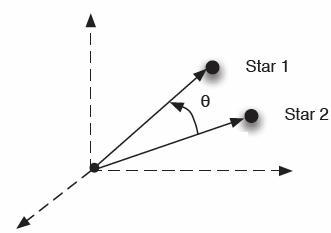
\includegraphics[scale=0.7]{vector_angle_method.jpg}
\centering
\caption{Vector angle method, Image \citet{gottlieb1978star}}
\label{fig:angle_matching}
\end{figure}

\citet{gottlieb1978star}
\begin{equation}
\theta = \cos^{-1}(\bm{r}_1 \cdot \bm{r}_2)
\end{equation}
\begin{equation}
\bm{b}_i = A\bm{r}_i
\end{equation}
\begin{equation}
\tilde{\bm{b}}_i = A\bm{r}_i + \bm{v}_i, \hspace{0.5cm} \bm{v}_i^TA\bm{r}_i = 0
\end{equation}
\begin{subequations}
\begin{equation}
E\left\{\bm{v}_i\right\} = 0
\end{equation}
\begin{equation}
E\left\{\bm{v}_i\bm{v}_i^T\right\} = \sigma_i^2 [\bm{I} - (A\bm{r}_i)(A\bm{r}_i)^T]
\end{equation}
\end{subequations}
\begin{equation}
\bm{b}_i^T\bm{b}_j = \bm{r}_i^TA^TA\bm{r}_j = \bm{r}_i^T\bm{r}_j
\end{equation}
\begin{subequations}
\begin{align*}
\tilde{\bm{b}}_i = A\bm{r}_i + \bm{v}_i\\
\tilde{\bm{b}}_j = A\bm{r}_j + \bm{v}_j
\end{align*}
\end{subequations}
\begin{equation}
z \equiv \tilde{\bm{b}}_i^T\tilde{\bm{b}}_j = \bm{r}_i^T\bm{r}_j + \bm{r}_i^TA^T\bm{v}_J + \bm{r}_j^TA^T\bm{v}_i + \bm{v}_i^T\bm{v}_j
\end{equation}
\begin{equation}
E\left\{z\right\} = \bm{r}_i^T\bm{r}_j
\end{equation}
\begin{equation}
p \equiv z - E\left\{z\right\} = \bm{r}_i^TA^T\bm{v}_J + \bm{r}_j^TA^T\bm{v}_i + \bm{v}_i^T\bm{v}_j
\end{equation}
\begin{equation}
\begin{split}
\sigma_p^2 \equiv E\left\{p\right\} = \\
\bm{r}_1^TA^TR_2A\bm{r}_1 + \bm{r}_2^TA^TR_aA\bm{r}_2 + Trace(R_1R_2) = \\
Trace(A\bm{r}_1\bm{r}_1^TR_2) + Trace(A\bm{r}_2\bm{r}_2^TR_1) + Trace(R_1R_2)
\end{split}
\end{equation}
\subsubsection{Spherical Triangle Matching}

\begin{figure}[ht]
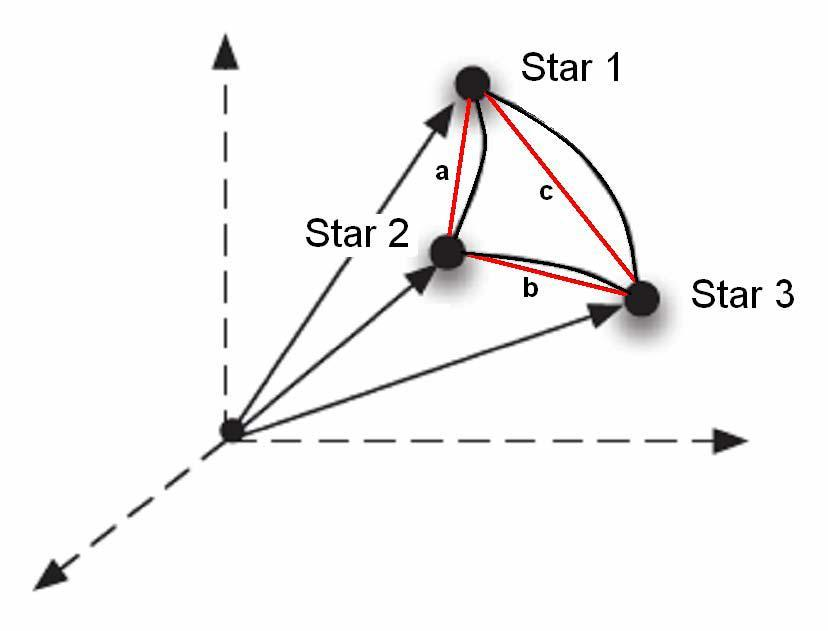
\includegraphics[scale=0.29]{spherical_triangle_method.jpg}
\centering
\caption{Spherical Triangle Method, Image \citet{cole2004fast}}
\label{fig:spherical_triangle_method}
\end{figure}

\citet{cole2004fast}

\begin{equation}
A = 4\tan^{-1}\sqrt{\tan\frac{s}{2}\tan\frac{s-a}{2}\tan\frac{s-b}{2}\tan\frac{s-c}{2}}
\end{equation}
\begin{subequations}
\begin{align*}
s = \frac{1}{2}(a + b + c) \\
a = \cos^{-1} \bigg(\frac{b_1 \cdot b_2}{|b_1||b_2|}\bigg) \\
b = \cos^{-1} \bigg(\frac{b_2 \cdot b_3}{|b_2||b_3|}\bigg) \\
c = \cos^{-1} \bigg(\frac{b_3 \cdot b_1}{|b_3||b_1|}\bigg) 
\end{align*}
\end{subequations}
\begin{equation}
I_p = \sum\theta^2dA
\end{equation}
\subsubsection{Planar Triangle}

\begin{figure}[ht]
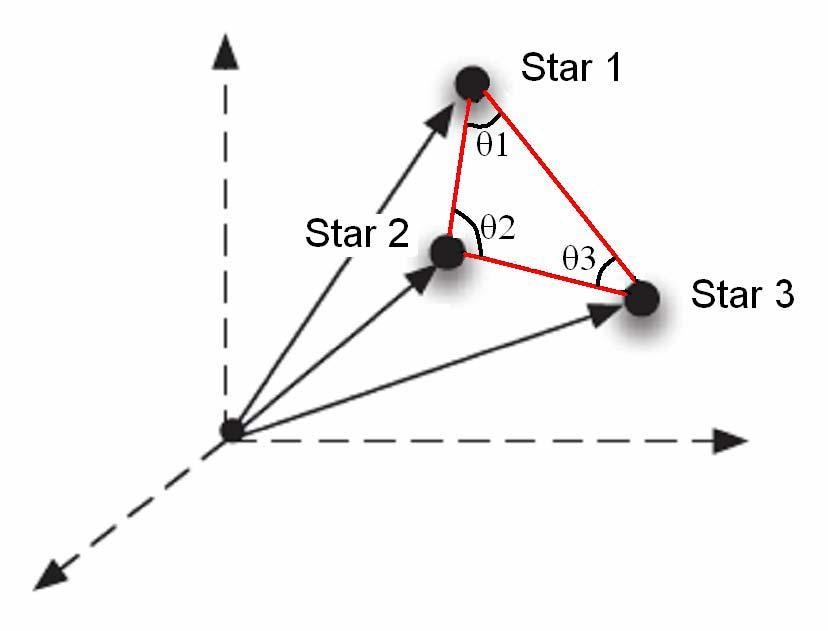
\includegraphics[scale=0.30]{planar_triangle_method.jpg}
\centering
\caption{Planar Triangle Method, Image \citet{cole2006fast}}
\label{fig:planar_triangle_method}
\end{figure}

\citet{cole2006fast}\par

\begin{subequations}
\begin{equation}
s = \frac{1}{2}(a + b + c)
\end{equation}
\begin{equation}
a = ||\bm{u_p} - \bm{u_q}||
\end{equation}
\begin{equation}
b = ||\bm{u_q} - \bm{u_r}||
\end{equation}
\begin{equation}
c = ||\bm{u_p} - \bm{u_r}||
\end{equation}
\end{subequations}
\begin{equation}
A = \sqrt{s(s-a)(s-b)(s-c)}
\end{equation}
\begin{equation}
J = A\frac{(a^2 + b^2 + c^2)}{36}
\end{equation}

Derivatives
\begin{equation}
H = \begin{bmatrix}
\bm{h}_1^T & \bm{h}_2^T & \bm{h}_3^T
\end{bmatrix}
\end{equation}

\begin{subequations}
\begin{equation}
\bm{h}_1^T \equiv \frac{\delta A}{\delta a}\frac{\delta a}{\delta\bm{b}_1} + \frac{\delta A}{\delta c}\frac{\delta c}{\delta\bm{b}_1}
\end{equation}
\begin{equation}
\bm{h}_2^T \equiv \frac{\delta A}{\delta a}\frac{\delta a}{\delta\bm{b}_2} + \frac{\delta A}{\delta b}\frac{\delta b}{\delta\bm{b}_2}
\end{equation}
\begin{equation}
\bm{h}_3^T \equiv \frac{\delta A}{\delta b}\frac{\delta b}{\delta\bm{b}_3} + \frac{\delta A}{\delta c}\frac{\delta c}{\delta\bm{b}_3} 
\end{equation}
\end{subequations}

\begin{subequations}
\begin{equation}
\frac{\delta A}{\delta a} = \frac{u_1 - u_2 + u_3 + u_4}{4A}
\end{equation}
\begin{equation}
\frac{\delta A}{\delta b} = \frac{u_1 + u_2 - u_3 + u_4}{4A}
\end{equation}
\begin{equation}
\frac{\delta A}{\delta c} = \frac{u_1 + u_2 + u_3 - u_4}{4A}
\end{equation}
\end{subequations}

\begin{subequations}
\begin{equation}
u_1 = (s - a)(s - b)(s - c)
\end{equation}
\begin{equation}
u_2 = s(s - b)(s - c)
\end{equation}
\begin{equation}
u_3 = s(s - a)(s - c)
\end{equation}
\begin{equation}
u_4 = s(s - a)(s - b)
\end{equation}
\end{subequations}

\begin{subequations}
\begin{equation}
\frac{\delta a}{\delta \bm{b}_1} = (\bm{b}_1 - \bm{b}_2)^T /a, \hspace{0.5cm} \frac{\delta a}{\delta \bm{b}_2} = -\frac{\delta a}{\delta \bm{b}_1}
\end{equation}
\begin{equation}
\frac{\delta b}{\delta \bm{b}_2} = (\bm{b}_2 - \bm{b}_3)^T /b, \hspace{0.5cm} \frac{\delta b}{\delta \bm{b}_3} = -\frac{\delta b}{\delta \bm{b}_2}
\end{equation}
\begin{equation}
\frac{\delta c}{\delta \bm{b}_1} = (\bm{b}_1 - \bm{b}_3)^T /c, \hspace{0.5cm} \frac{\delta c}{\delta \bm{b}_3} = -\frac{\delta c}{\delta \bm{b}_1}
\end{equation}
\end{subequations}

\begin{equation}
\sigma_A^2 = HRH^T
\end{equation}

\begin{equation}
R \equiv \begin{bmatrix}
R_1 & 0_{3x3} & 0_{3x3} \\
0_{3x3} & R_2 & 0_{3x3} \\
0_{3x3} & 0_{3x3} & R_3
\end{bmatrix}
\end{equation}

Polar Moment

\begin{equation}
\bar{H} = \begin{bmatrix}
\bar{\bm{h}}_1^T & \bar{\bm{h}}_2^T & \bar{\bm{h}}_3^T
\end{bmatrix}
\end{equation}

\begin{subequations}
\begin{equation}
\bar{\bm{h}}_1^T \equiv \frac{\delta J}{\delta a}\frac{\delta a}{\delta\bm{b}_1} + \frac{\delta J}{\delta c}\frac{\delta c}{\delta\bm{b}_1} + \frac{\delta J}{\delta A}\bm{h}_1^T
\end{equation}
\begin{equation}
\bar{\bm{h}}_2^T \equiv \frac{\delta J}{\delta a}\frac{\delta a}{\delta\bm{b}_2} + \frac{\delta J}{\delta b}\frac{\delta b}{\delta\bm{b}_2} + \frac{\delta J}{\delta A}\bm{h}_2^T
\end{equation}
\begin{equation}
\bar{\bm{h}}_3^T \equiv \frac{\delta J}{\delta b}\frac{\delta b}{\delta\bm{b}_3} + \frac{\delta J}{\delta c}\frac{\delta c}{\delta\bm{b}_3} + \frac{\delta J}{\delta A}\bm{h}_3^T
\end{equation}
\end{subequations}

\begin{subequations}
\begin{equation}
\frac{\delta J}{\delta a} = A a/18, \hspace{0.5cm} \frac{\delta J}{\delta a} = A b/18, \hspace{0.5cm} \frac{\delta J}{\delta a} = A c/18
\end{equation}
\begin{equation}
\frac{\delta J}{\delta A} = (a^2 + b^2 + c^2)/36
\end{equation}
\end{subequations}

\begin{equation}
\sigma_J^2 = \bar{H}R\bar{H}^T
\end{equation}

\subsubsection{Pyramid}

\begin{figure}[ht]
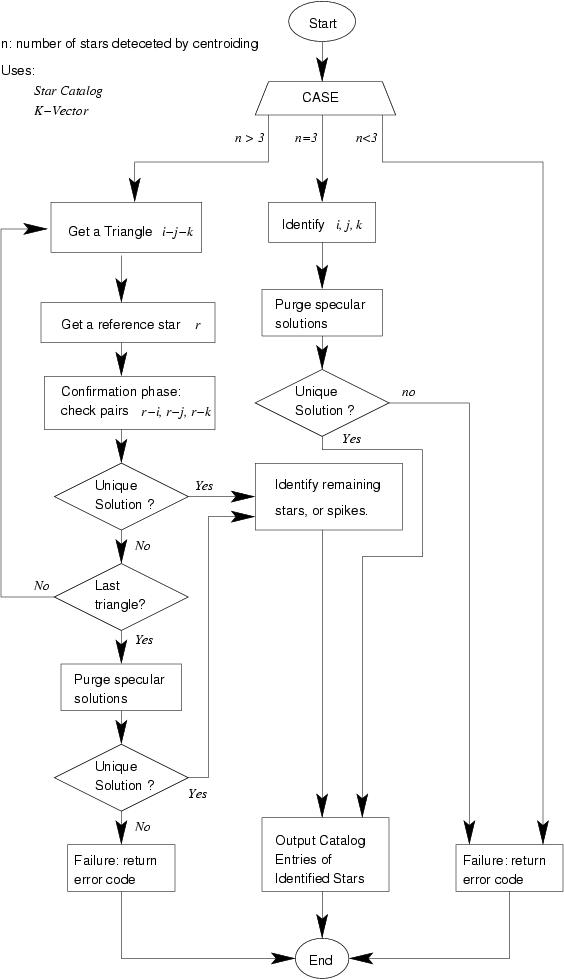
\includegraphics[scale=0.57]{pyramid_method.jpg}
\centering
\caption{Pyramid Method Flowchart, Image \citet{mortari2004pyramid}}
\label{fig:pyramid_method}
\end{figure}

\citet{mortari2004pyramid}\par


\subsubsection{Rate Matching}
\citet{samaan2005recursive}
to be removed?
\subsubsection{Voting}
\citet{kolomenkin2008geometric} \par
\subsubsection{Grid}
%http://dsp.ucsd.edu/~kreutz/Publications/Padgett1997.pdf
\citet{padgett1997grid}
\subsection{Star-catalogue and searching for matching stars}

\subsubsection{Star Catalogue Generation}
\citet{6187242}
\begin{equation}
\bm{u} = \begin{bmatrix}
\cos \alpha \cos \delta \\
\sin \alpha \cos \delta \\
\sin \delta
\end{bmatrix}
\end{equation}
\begin{equation}
m_i \leq m_{max}
\end{equation}
\begin{equation}
m_j \leq m_{max}
\end{equation}
\begin{equation}
\bm{u_a^T u_b} \geq \cos \theta_{FOV}
\end{equation}

\subsubsection{Candidate Matching}
to be removed?
\subsubsection{Result Verification}
to be removed?
\subsubsection{k-vector}
The k-vector database is built a priori for some given working
magnitude threshold and for the star tracker maximum angular aperture. Essentially, the k-vector table is a structural database of all catalogued star pairs that could possibly fit in the camera FOV over the whole sky. The star pairs are ordered with increasing inter-star angle.
The data stored are the k index, the cosine of the interstar angle, and the master catalogue indices I[k] and J[k] of the kth star pair. The k-vector access logic is invoked in real time for a minimal set of star pairs in elementary measured star polygons (three for a triangle, six for a four-star pyramid, etc.); the fact that the vertices between adjacent measured star pairs share a common catalogued star is the key observation leading to logic for efficiently identifying the stars by simply comparing the k-vector accessed catalogue indices from the several sets of candidate star pairs (which must contain the common measured pivot star, if
it is in the catalog).
\citet{mortari2013k}\par
\citet{mortari1996fast}\par
\citet{mortari2000k}\par
Trzeba dodać pogrubienia vectorów
\begin{equation}
z(x) = mx + q
\end{equation}
\begin{equation}
m = \frac{y_{max} - y_{min} + \delta\epsilon}{n - 1}
\end{equation}
\begin{equation}
q = y_{min} - m - \delta\epsilon
\end{equation}
\begin{equation}
\epsilon \approx 22.2 \times 10^{-16}
\end{equation}
\begin{equation}
\delta\epsilon = (n - 1)\epsilon
\end{equation}
\begin{equation}
k(i) = j \hspace{0.5cm} where \hspace{0.5cm} s(j) \leq z(i) < s(j + 1)
\end{equation}
or
\begin{equation}
k(i) = j \hspace{0.5cm} \textnormal{where j is the greatest index such} \hspace{0.5cm} s(j) \leq y(I(i)) \hspace{0.5cm} \textnormal{is satisfied.}
\end{equation}
\begin{equation}
j_b = \Big\lfloor\frac{y_a - q}{m}\Big\rfloor \hspace{0.5cm} and \hspace{0.5cm} j_t = \Big\lceil\frac{y_b - q}{m}\Big\rceil
\end{equation}
\begin{equation}
k_{start} = k(j_b) + 1 \hspace{0.5cm} and \hspace{0.5cm} k_{end} = k(j_t)
\end{equation}
\subsection{Attitude Determination}
\citet{jenssen2011comparison}\par
AIM (Attitude estimation using Image Matching)\citet{delabie2012highly}\par
all \citet{hall2003spacecraft} \citet{markley1999estimate}
\subsubsection{q-method}

\begin{equation}
\bm{s}_b = \bm{R}^{bi}\bm{s}_i \hspace{0.5cm} \bm{m}_b = \bm{R}^{bi}\bm{m}_i
\end{equation}

\begin{equation}
\begin{split}
J &= \frac{1}{2} \sum w_k (\bm{v}_{kb} - \bm{R}^{bi} \bm{v}_{ki})^T (\bm{v}_{kb} - \bm{R}^{bi} \bm{v}_{ki}) \\ 
&= \frac{1}{2} \sum w_k (\bm{v}_{kb}^T\bm{v}_{kb} + \bm{v}_{ki}^T\bm{v}_{ki} + 2\bm{v}_{kb}^T \bm{R}^{bi} \bm{v}_{ki})
\end{split}
\end{equation}


\begin{equation}
J = \sum w_k (1 - \bm{v}_{kb}^T \bm{R}^{bi} \bm{v}_{ki})
\end{equation}

\begin{equation}
g(\bm{R}) = \sum w_k \bm{v}_{kb}^T \bm{R}^{bi} \bm{v}_{ki}
\end{equation}

\begin{equation}
\bm{R} = (q_4^2 - \bm{q}^T\bm{q})1 + 2\bm{qq}^T - 2q_4\bm{q}^{\bm{x}}
\end{equation}

\begin{equation}
\bm{\bar{q}}^T\bm{\bar{q}} = 1
\end{equation}

\begin{equation}
g(\bm{\bar{q}}) = \bm{\bar{q}}^T\bm{K}\bm{\bar{q}}
\end{equation}

\begin{equation}
\bm{K} = \begin{bmatrix}
\bm{S} - \sigma\bm{I} & \bm{Z} \\
\bm{Z}^T & \sigma
\end{bmatrix}
\end{equation}

\begin{equation}
\bm{B} = \sum_{k=1}^Nw_k(\bm{v}_{kb}\bm{v}_{ki}^T)
\end{equation}

\begin{equation}
\bm{S} = \bm{B} + \bm{B}^T
\end{equation}

\begin{equation}
\bm{Z} = \begin{bmatrix}
B_{23} - B_{32} & B_{32} - B_{13} & B_{12} - B_{21}
\end{bmatrix} ^T
\end{equation}

\begin{equation}
\sigma = tr[\bm{B}]
\end{equation}

\begin{equation}
g'(\bm{\bar{q}}) = \bm{\bar{q}}^T\bm{K}\bm{\bar{q}} - \lambda\bm{\bar{q}}^T\bm{\bar{q}}
\end{equation}

\begin{equation}
\bm{K}\bm{\bar{q}} = \lambda\bm{\bar{q}}
\end{equation}

\begin{equation}
g(\bm{\bar{q}}) = \bm{\bar{q}}^T\bm{K}\bm{\bar{q}} = \bm{\bar{q}}^T\lambda\bm{\bar{q}} = \lambda\bm{\bar{q}}^T\bm{\bar{q}} = \lambda
\end{equation}

\subsubsection{Wahba's problem}

The developed extended QUEST method described in this report builds upon the principles
of Wahba’s problem. The problem was first stated by Grace Wahba in 1965 \citet{wahba1965least}. Given
two sets of vector observations, a rotation matrix $\bm{M}$ can be found which minimizes the
orientation error. This is an optimization problem, where the cost function is:

\begin{equation}
\sum_j^n ||\bm{r}_j - \bm{Mb}_j||
\end{equation}

For satellite attitude determination, the vectors $\bm{r}_j$ for $j \in \left\{1, n\right\}$ are the reference sensor data given in the NED frame. The vectors $\bm{b}_j$ for $j \in \left\{1, n\right\}$  are the measured sensor data in the BODY frame. $\bm{M}$ is the least squares estimate of the rotation matrix which carries the known frame of reference into the satellite fixed frame of reference.
The QUEST method uses this problem in order to minimize the attitude estimation error.
\subsubsection{QUEST}
improvement to quest implementation \citet{RIS_1} \par
kallman filtering \citet{shuster1990kalman}
\begin{equation}
\begin{split}
J(\bm{q}) = \frac{1}{2}\sum_{j=1}^n\frac{1}{\sigma_j^2}(\bm{b}_j - \bm{R}_b^i(\bm{q})\bm{r}_j)^T(\bm{b}_j - \bm{R}_b^i(\bm{q})\bm{r}_j) = \\
\frac{1}{2}\sum_{j=1}^n\frac{1}{\sigma_j^2}(\bm{b}_j^T\bm{b}_j - 2\bm{b}_j^T\bm{R}_b^i(\bm{q})\bm{r}_j + \bm{r}_j^T\bm{r}_j)
\end{split}
\end{equation}
\begin{equation}
J(\bm{q}) = \sum_{j=1}^n\frac{1}{\sigma_j^2}(1 - \bm{b}_j^T\bm{R}_b^i(\bm{q})\bm{r}_j)
\end{equation}
\subsubsection{TRIAD}
a must
\subsubsection{The Fast Optimal Attitude Matrix}
to be removed?
\subsubsection{DCM (Direction Cosine Matrix)}
\citet{juang2003efficient}
 and

\citet{6187242}
\begin{equation}
\bm{B = \sum_{i=1}^nb_ir_i^T}
\end{equation}
\begin{equation}
\bm{B = USV^T}
\end{equation}
\begin{equation}
\bm{U}_+ = \bm{U}\begin{bmatrix}
1 & 0 & 0 \\
0 & 1 & 0 \\
0 & 0 & det\bm{U}
\end{bmatrix}
\end{equation}
\begin{equation}
\bm{V}_+ = \bm{V}\begin{bmatrix}
1 & 0 & 0 \\
0 & 1 & 0 \\
0 & 0 & det\bm{V}
\end{bmatrix}
\end{equation}
\begin{equation}
\bm{A = U_+V_+^T}
\end{equation}
\newpage
\section{Prototype}
For now the following parts are finished in Python:
\begin{enumerate}
\item Centroiding
\item Planar Triangle Recognition with variations (nearly - without equation 44)
\item Pyramid alg ?
\item k-vector
\item QUEST (not started yet)
\end{enumerate}
Testing\par
\citet{kruijff2003star}
\newpage
\section{Complete program}

\newpage
\section{Testing of star-tracker}
\citet{RIS_0}

\newpage
\bibliographystyle{IEEEtranN}
\bibliography{IEEEabrv,bibfile}
%\bibliography{bibfile}




\newpage

\listoftables

\newpage

\listoffigures

\newpage


\end{document}
